\section{不同架构间的核心对比参数}

本章将深入探讨影响GPU性能的关键参数。理解这些内容将有助于我们后续阅读GPU白皮书和数据手册。

从前几章中，我们已知每一代新架构都在软件和硬件能力上带来了显著进步，在各类领域和应用中提供了更高的性能。一个清晰的例子就是
从 Fermi 架构到 Hopper 架构的吞吐量增长，如下表所示，吞吐量增长超过了300倍。

如果你还记得前文关于 GPU 性能的重要提示，评估性能并非一目了然，它需要理解数十种指标和单位，而不仅仅是吞吐量或速度。
那么，有哪些参数、单位和指标可用于衡量每一代新架构相较于前代的性能？例如，当 NVIDIA 在新架构中增加核心数量时，这是否
足以提升架构性能，还是存在其他因素？为回答这个问题，让我们来看这些关键参数和指标——它们是理解 GPU 性能最关键的要素，
但需注意，它们并非评估 GPU 性能的全部指标，只是最主要的几个。

\subsection{内存带宽}

本章的第一个参数是内存带宽。内存带宽指的是内存每秒能处理多少数据，以 GB/s（每秒千兆字节）来衡量。为了说明内存带宽对应用
性能的影响，我们来讨论以下场景。假设我们有一块 GPU，其全局内存提供的带宽有限。再假设该 GPU 包含四个核心，而这块内存每
秒只能提供 32 位数据。每个核心都需要从该内存读取 32 位数据，所需数据总量为 128 位。那么问题是：这块内存能否在一秒内处理
全部四个请求？

\begin{figure}
    \centering
    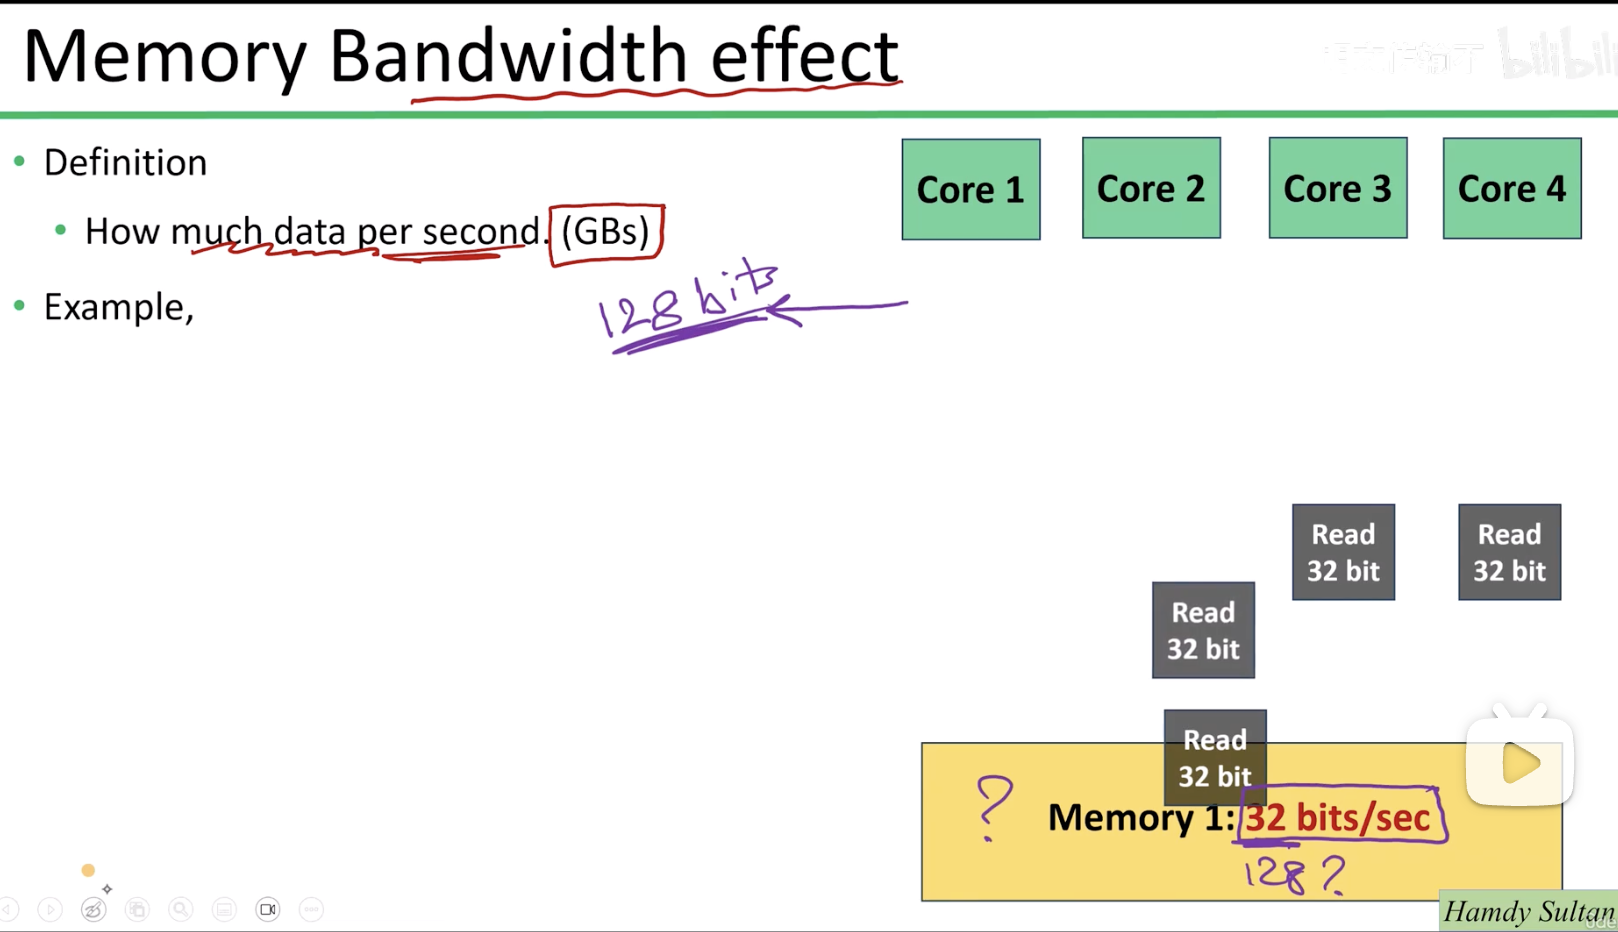
\includegraphics[width=0.75\linewidth]{resources/cuda-025.png}
    \caption{带宽}
    \label{fig:placeholder}
\end{figure}


不幸的是，答案是否定的。由于最大带宽为每秒32位，该内存一次只能处理一个请求。它在第一秒处理第一个请求（前32位），完成后
再继续下一个请求，依此类推。这种串行处理意味着内存需要总共4秒才能响应所有读取请求。

\begin{figure}
    \centering
    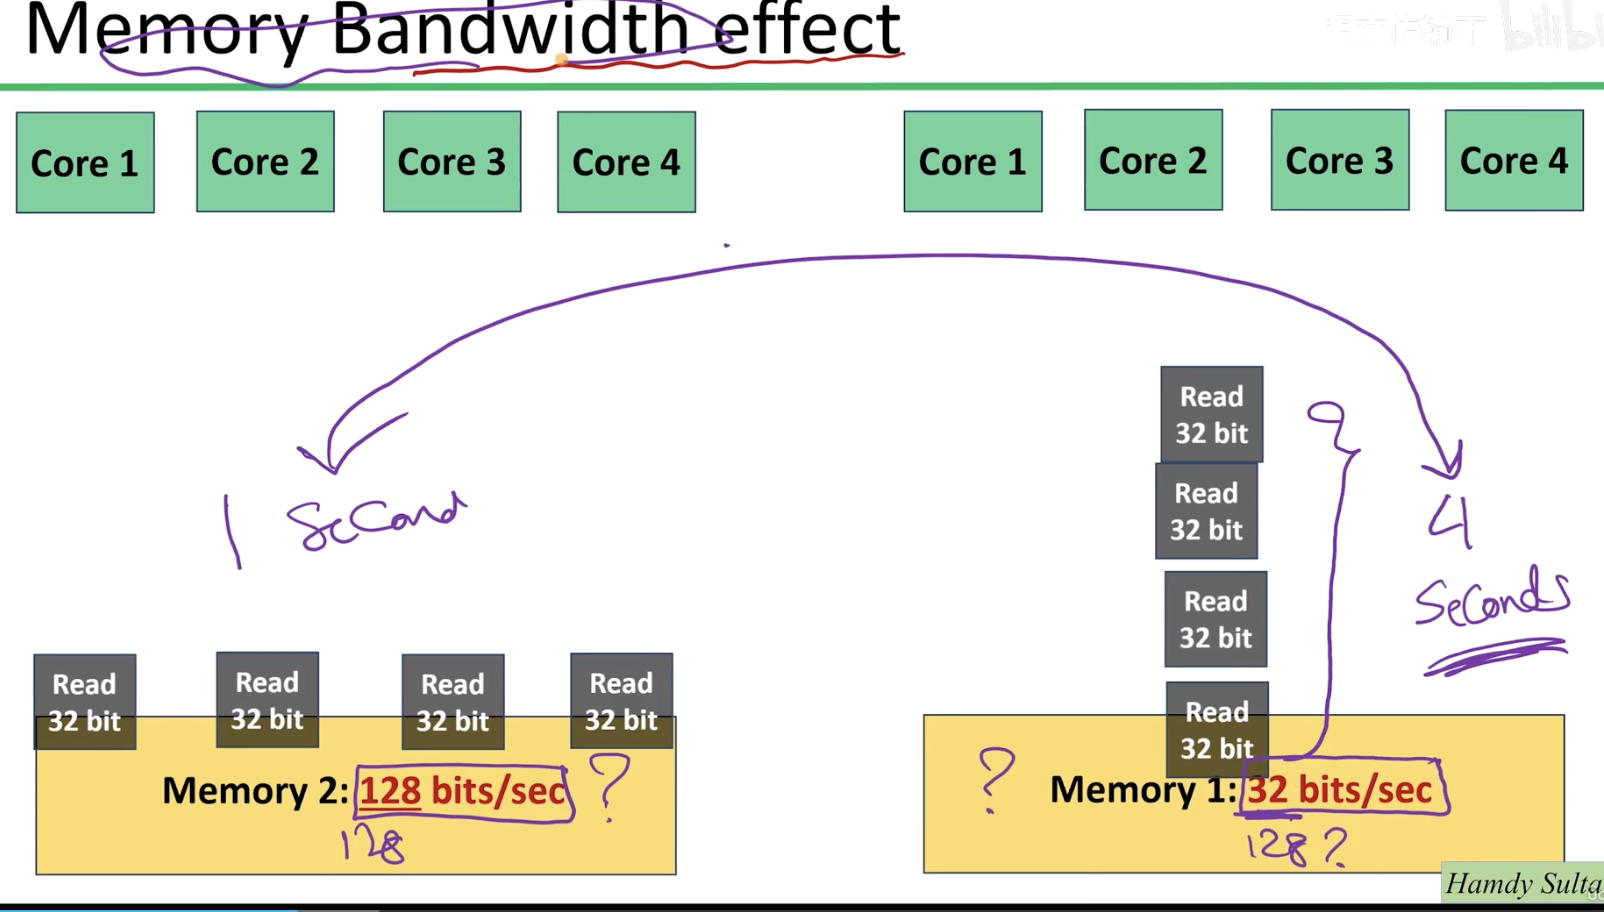
\includegraphics[width=0.75\linewidth]{resources/cuda-026.png}
    \caption{带宽}
    \label{fig:placeholder}
\end{figure}


现在我们将其与另一种带宽更高的内存进行比较。假设我们有一块带宽为每秒128位的内存，同样有来自四个核心的四个读取请求。该
内存的更高带宽可以在一秒内传输128位，这意味着它能在一秒内响应全部四个请求。这充分说明了内存带宽在提升GPU性能中的关键
作用——相比第一块内存，高带宽显著减少了读写操作所需的时间。

从实际角度来看，考虑视频编辑或三维渲染这类带宽密集型应用，更高的内存带宽会使这些应用或任务效率显著提升。在游戏领域，每一
毫秒都至关重要，更高的内存带宽意味着更流畅的帧率和更沉浸的体验，同时也有助于减少延迟。总结一下，更高的带宽使GPU能一次
处理更多数据，从而提升性能。

你可能会疑惑，为什么这里的带宽会与内存速度和总线宽度并列？答案是这两个因素会直接影响内存带宽。为说明这一点，让我们深入看
看总线宽度对内存带宽的影响。


\subsection{总线宽度}

计算机架构中总线宽度的概念可以类比为道路上的车道数量。如果我们把每份数据看作一辆汽车，那么总线宽度就是这些汽车可通行的车
道数量。考虑两种不同场景：第一种场景假设我们有2位总线宽度，相当于一条双车道的道路，因此一次能通过检查点的汽车数量是两辆
。如果每条车道的限速是每秒一辆车，那么在道路尽头的检查点，一秒内总共能通过的汽车数量就是两辆——因为有两条车道，每条车道
每秒一辆车。

\begin{figure}
    \centering
    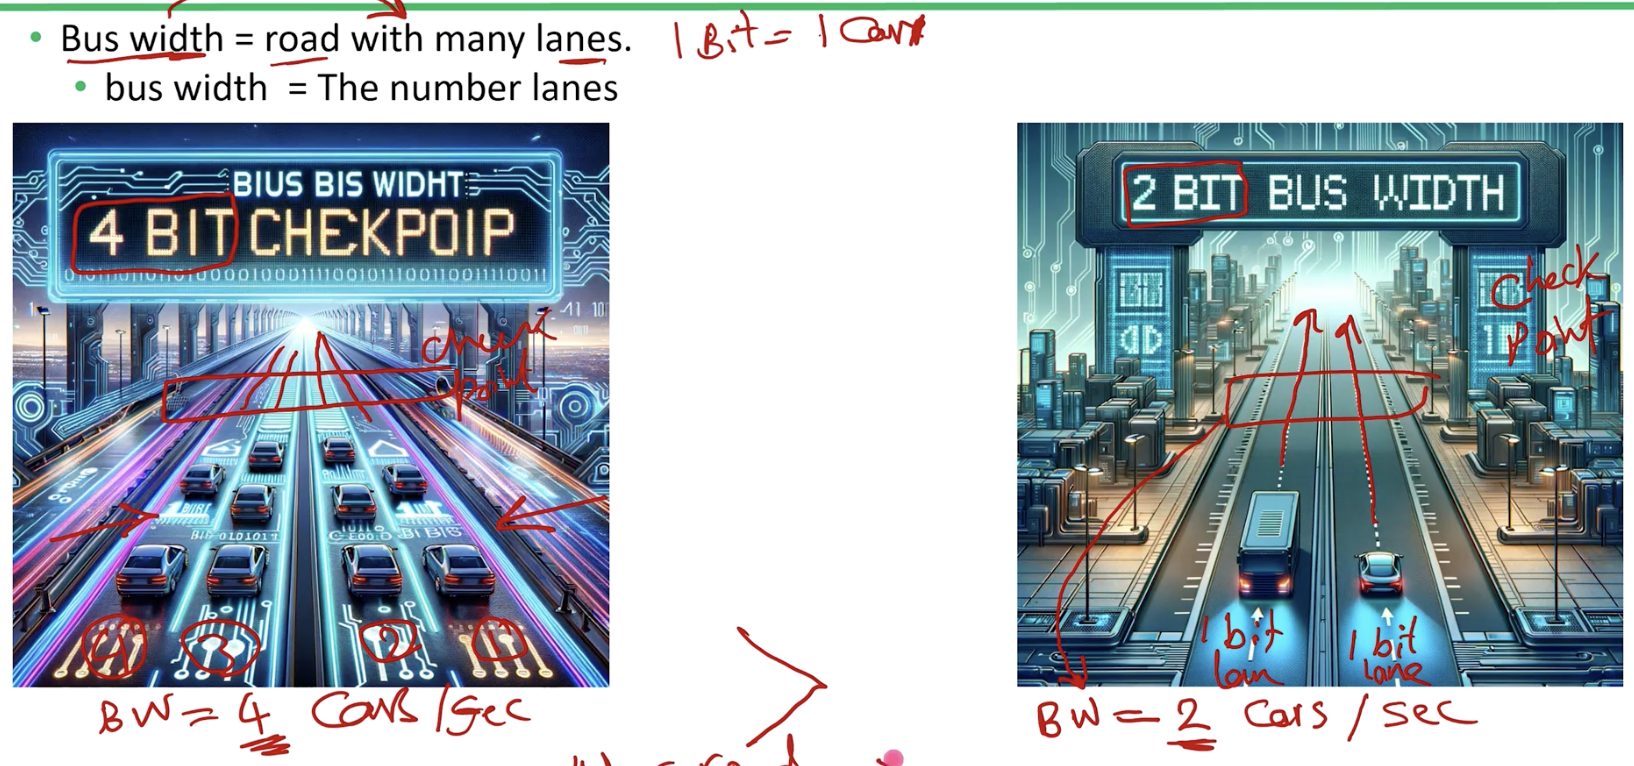
\includegraphics[width=0.75\linewidth]{resources/cuda-027.png}
    \caption{带宽}
    \label{fig:placeholder}
\end{figure}


这条路可让两辆车同时通过检查点，该检查点的带宽是每秒两辆车。第二个例子，假设我们有4位总线宽度，即一条四车道道路。采用相同的限速（每秒一辆车），这条路每秒能处理四辆车。第一条路（2
位总线）的带宽是每秒两辆车，第二条路（4位总线）的带宽是每秒四辆车。总结这两个例子：更宽的总线宽度带来更高的带宽。

现在让我们回到计算机术语，应用同样的类比：将总线宽度翻倍，例如从32位提升到64位，会增加在给定时间内可传输的数据量。但
这仅在内存速度相同的情况下才成立。在同样语境下，内存速度通常称为内存时钟频率，也是GPU性能的关键因素。更高的内存速度使
GPU能更快地访问和处理数据，从而减少瓶颈。关键不仅在于可用内存有多少，更在于内存运行得多快，这对数据密集型任务的整体效
率至关重要。

在之前的类比中，假设每条车道由一名警官管理。检查点的效率不仅取决于道路宽度（车道数量），还关键取决于每名警官检查一辆车的
速度有多快。如果每名警官工作效率更高，能更快地检查每辆车，自然就能在给定时间内让更多车辆通过检查点。

这个类比直接对应GPU中内存的工作方式。如果内存具备更高的速度，就能在特定时间范围内处理更多数据、事务或操作，从而有效提
升内存带宽。正如检查点上效率更高的警官能带来更顺畅、更高效的车流，GPU中更高的内存速度也会带来更大的内存带宽。这种增强
的带宽对GPU整体性能至关重要，因为它决定了数据从内存传输到计算单元（核心）的速度有多快。

\begin{figure}
    \centering
    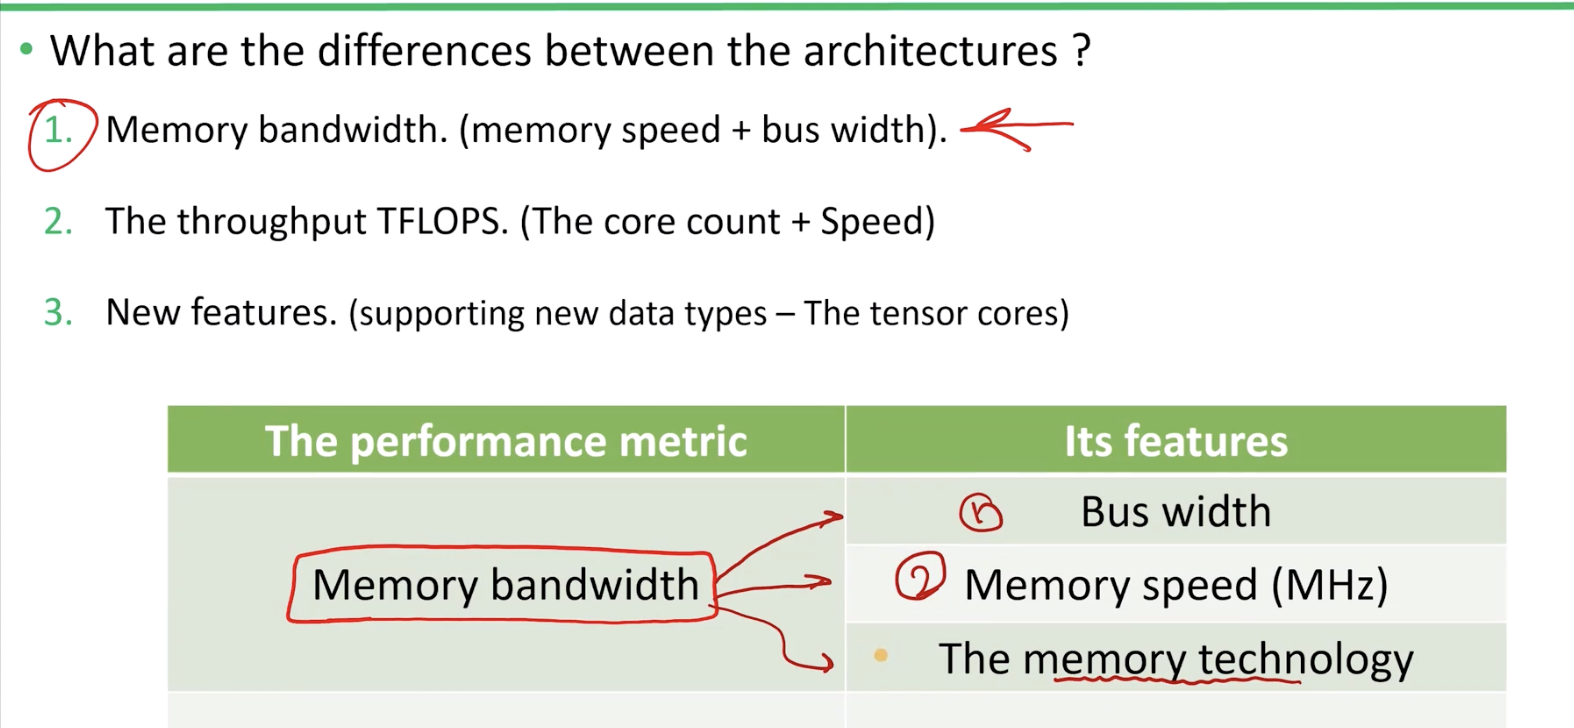
\includegraphics[width=0.75\linewidth]{resources/cuda-028.png}
    \caption{带宽}
    \label{fig:placeholder}
\end{figure}


我们在此考察的指标是内存带宽。现在来总结一下：该指标会受到不同因素的影响，例如内存速度、内存总线宽度以及内存技术（DDR4、
DDR5、DDR6，甚至更新的HBM等）。现在让我们在两款属于不同类别的GPU上检验这一指标及其影响因素。这两款GPU分别是
来自Tesla系列的A100和来自GeForce系列的RTX 3090，如果你还记得我们之前的讨论，Tesla系列专用于高性能计算，而
GeForce则面向游戏和普通用户。需要再次指出的是，这两款GPU都基于Ampere架构，因此它们共享相同的架构，但面向不同的应用场景。

\begin{figure}
    \centering
    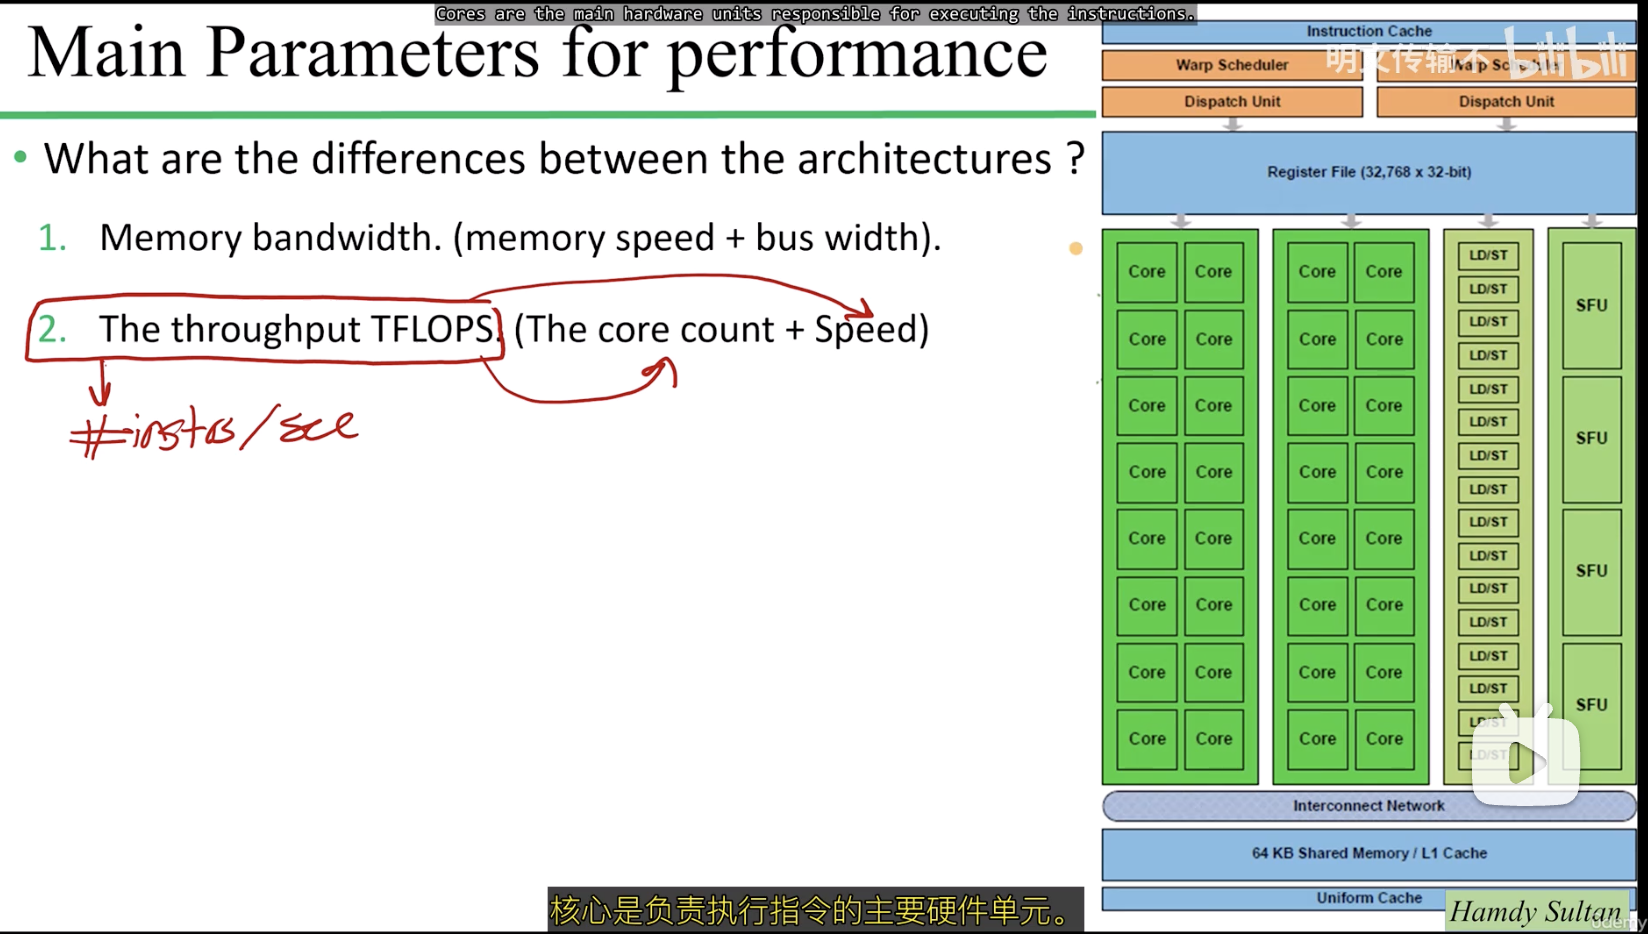
\includegraphics[width=0.75\linewidth]{resources/cuda-029.png}
    \caption{带宽}
    \label{fig:placeholder}
\end{figure}


在高性能计算A100 GPU中，我们观察到其内存总线宽度异常宽——超过5000位，即5000条车道。为便于理解，我们将此数值与
RTX 3090的总线宽度进行比较。尽管共享相同架构，RTX 3090 GPU的总线宽度却只有约400位。你看到差别了吗？A100是5000
位，而RTX 3090只有400位，两者差距超过十倍。此外，当考察内存速度时，它们大致相当。但当我们综合这些因素——内存速度、
总线宽度以及内存技术——就会发现A100 GPU在内存带宽方面显著优于RTX 3090。

在A100中，我们使用了名为HBM2的内存技术，而在RTX 3090中则使用了另一种名为GDDR6的技术。
在介绍下一个参数之前，先思考一个问题：你认为 GPU 中包含的核心数量是否直接影响其性能？来看一个例子，假设需要比较两
款GPU，第一款有100个核心，第二款有200个核心。我们能否说第二款性能更好？

\begin{figure}
    \centering
    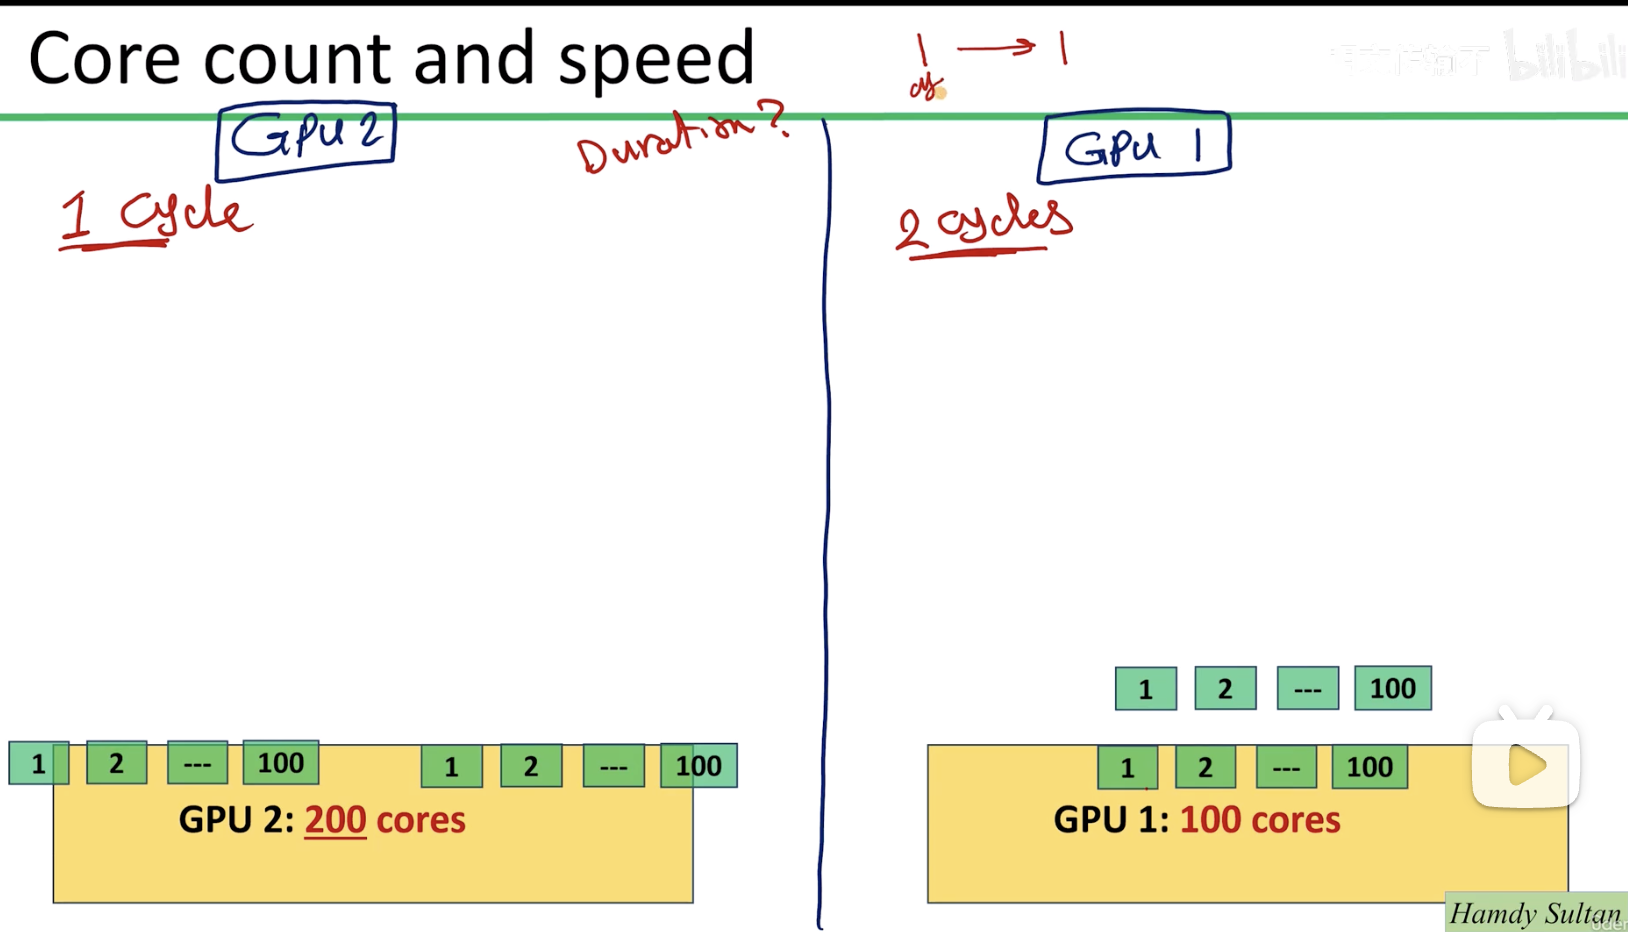
\includegraphics[width=0.75\linewidth]{resources/cuda-030.png}
    \caption{带宽}
    \label{fig:placeholder}
\end{figure}

\subsection{指令吞吐量}

我将通过讲解第二个参数——指令吞吐量——来回答这个问题。在此上下文中，吞吐量指的是整个GPU每秒执行的指令总数。该指
标直接受两个因素影响：核心数量和核心速度，是评估和比较不同GPU型号的关键度量。

为更深入理解这一概念，让我们考虑GPU中核心的作用。核心是负责执行指令的主要硬件单元，更多的核心允许同时执行更多指令，从
而带来更高的吞吐量。为具体说明，假设有两款不同的GPU，一款配备100个核心，另一款配备200个核心。再假设有一个包含200条
指令的应用程序，当该应用程序在两款GPU上运行时，第一款GPU将为每个核心分配一条指令，在第一个周期中处理100条指令，然
后将剩下的100条指令再次分配给各核心。


在第二款GPU的场景中，200条指令将在一个周期内执行完毕，因为我们有200个核心，每个核心接收一条指令。这使得GPU仅用一个
周期而非两个就能完成整个应用程序，性能相较第一款GPU提升了一倍。更高的核心数量意味着更强的并行处理能力，从而实现更快、
更高效的任务执行，尤其适用于可有效并行化的应用程序。这个例子突显了核心数量对GPU吞吐量的重大影响，但这并非绝对真理——在
某些情况下，第一款GPU（核心更少）的性能可能优于第二款GPU。

\begin{figure}
    \centering
    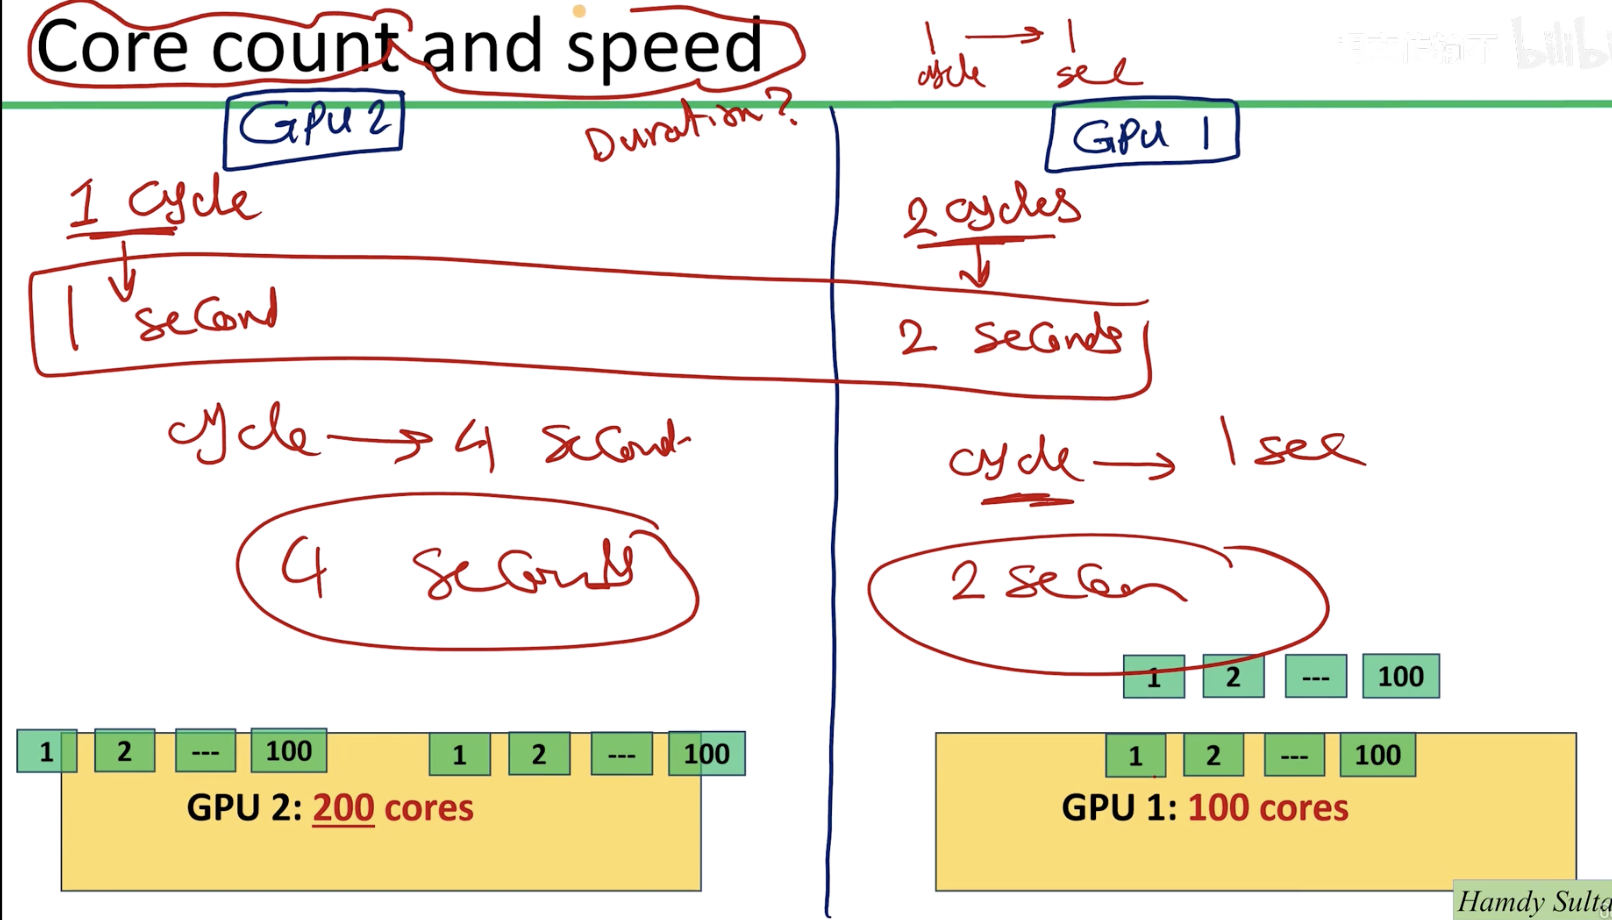
\includegraphics[width=0.75\linewidth]{resources/cuda-031.png}
    \caption{带宽}
    \label{fig:placeholder}
\end{figure}

让我们回顾这个例子：第一款GPU需要两个周期来执行整个应用程序，而第二款GPU只需一个周期。然而，如果我们不知道两款GPU中
每个周期的持续时间，我们的比较就缺乏上下文。为说明这一点，再考虑一个假设：如果第一款GPU每个周期耗时1秒，而第二款GPU
每个周期耗时4秒呢？在这种情况下，第一款GPU将在2秒内完成，而第二款GPU需要4秒。


这一场景凸显了GPU架构中的一个关键方面：核心数量与核心时钟频率之间的平衡。时钟频率——即每个核心执行指令的速率——同样至
关重要。核心数量确实影响同时处理多条指令的能力，这是GPU并行处理的基本原则。但更高的时钟频率意味着每个核心能更快完成分
配的任务，这在需要快速处理复杂小任务的应用中尤为关键。我们可以通过吞吐量这一指标——即单位时间内可执行的指令数量（如每秒
）——来衡量它们对性能的综合影响。

\begin{figure}
    \centering
    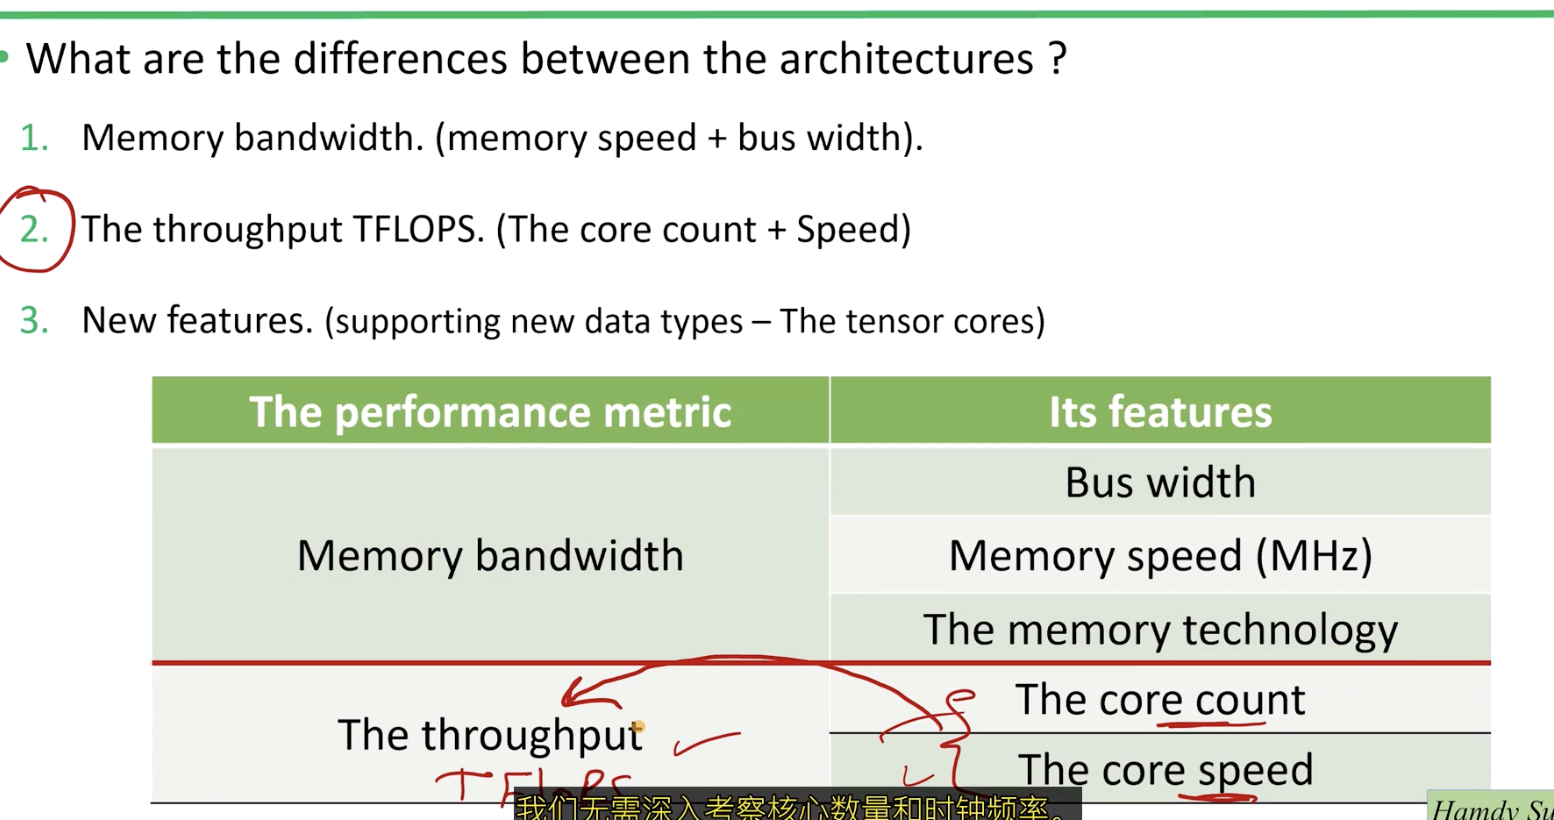
\includegraphics[width=0.75\linewidth]{resources/cuda-032.png}
    \caption{带宽}
    \label{fig:placeholder}
\end{figure}

总结一下，核心数量加上核心速度是重要的硬件特性。在查阅白皮书或数据手册时，我们可以直接关注吞吐量指标，而不必深入考察核心
数量。它们固然重要，但关注吞吐量可以绕过对核心数量和时钟频率的逐一分析。不过时钟频率始终对能耗有重要影响。

\subsection{能耗权衡}

让我们探讨另一个关键问题——这一点非常重要。假设我们有两款 GPU，第一款 GPU 不仅核心数量更多、核心频率更高，其运行速度
也快于第二款。第一款 GPU 在核心数量和速度上都强于第二款，这是否自动使其成为更优选择？根据之前的讨论，你可能会初步认为：
更多的核心、更高的速度，还需要什么呢？

然而，还有另一个关键因素需要考虑——能耗。更高的速度加上更多的核心数量会导致更高的能耗。如果一家公司优先考虑能效（这通常
与节省成本相关），它可能会选择第二款GPU，尽管其规格较低。这一场景体现了一种权衡：如果你想要更高的计算能力和速度，就
必须承担更高的能耗成本，反之亦然。如果我问你哪款GPU更优越，你的回答应该是一个反问——在什么上下文中？你是考虑能效还是
计算能力？

评估GPU性能时，最后一个要考虑的参数是新架构中引入的新特性或硬件单元。


\begin{figure}
    \centering
    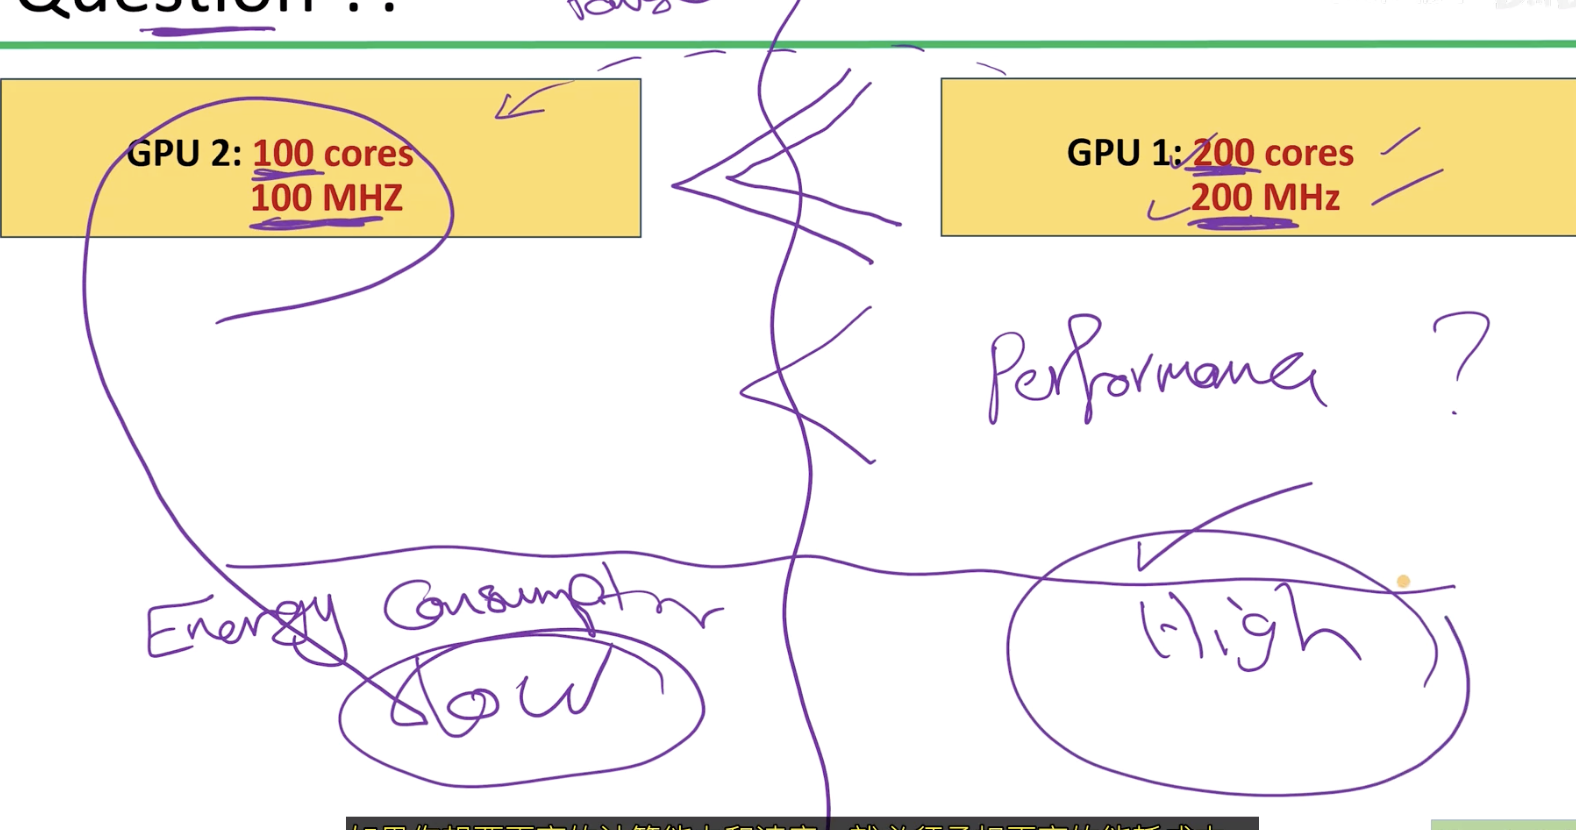
\includegraphics[width=0.75\linewidth]{resources/cuda-033.png}
    \caption{带宽}
    \label{fig:placeholder}
\end{figure}

\subsection{新特性}

有时一个新单元能显著增强GPU的计算能力。例如，NVIDIA在2017年推出的Volta架构中加入了张量核心（Tensor Core）。请看这张
图，它展示了从Pascal到Volta的性能飞跃——同一应用的性能大约提升了八倍。请想象一个复杂的人工智能应用，通常需要消耗八天的
计算资源；而在Volta架构中，借助张量核心，同样的任务可能只需一天即可完成。这个例子突显了张量核心作为硬件单元在GPU计算领
域中的革命性影响。顺便一提，本课程中有专门章节讲解张量核心及其使用方法。

\begin{figure}
    \centering
    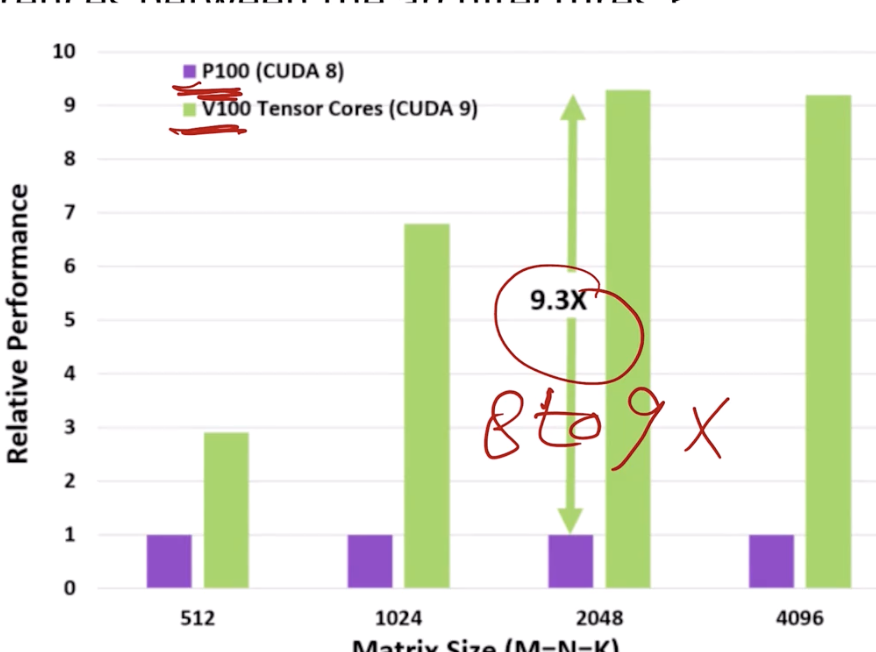
\includegraphics[width=0.75\linewidth]{resources/cuda-034.png}
    \caption{带宽}
    \label{fig:placeholder}
\end{figure}

本章最后，让我们来看一下 NVIDIA 所有白皮书和数据手册中都存在的一张表格。在这张表格中你会注意到列出了大量特性和指标——这
些行提供了关于各种数据类型（从浮点到整数运算）的核心数量信息。然而，正如我们讨论过的，仅看核心数量可能无法全面反映情况
：理解核心速度与核心数量同样重要。或者我们可以直接关注指令吞吐量来简化分析，该指标以 TFLOPS（每秒万亿次浮点运算，即 
\(10^{12}\) 次浮点运算/秒）来衡量。在接下来的章节中，我们将基于本章的讨论，深入探讨最新 GPU 的规格，这些规格来自白皮书和
数据手册中的架构信息。

\begin{figure}
    \centering
    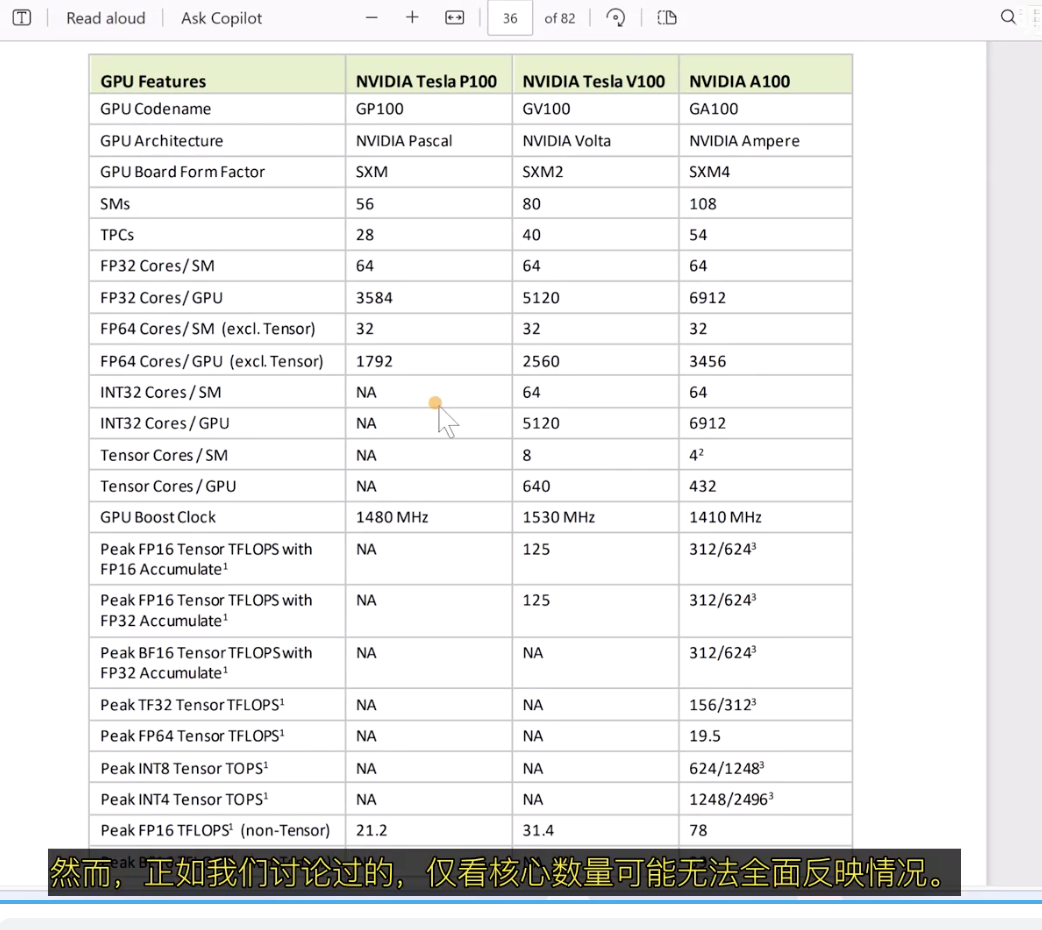
\includegraphics[width=0.75\linewidth]{resources/cuda-035.png}
    \caption{性能数据}
    \label{fig:placeholder}
\end{figure}
